\documentclass[12pt]{article}\usepackage[]{graphicx}\usepackage[]{color}
%% maxwidth is the original width if it is less than linewidth
%% otherwise use linewidth (to make sure the graphics do not exceed the margin)
\makeatletter
\def\maxwidth{ %
  \ifdim\Gin@nat@width>\linewidth
    \linewidth
  \else
    \Gin@nat@width
  \fi
}
\makeatother

\definecolor{fgcolor}{rgb}{0.345, 0.345, 0.345}
\newcommand{\hlnum}[1]{\textcolor[rgb]{0.686,0.059,0.569}{#1}}%
\newcommand{\hlstr}[1]{\textcolor[rgb]{0.192,0.494,0.8}{#1}}%
\newcommand{\hlcom}[1]{\textcolor[rgb]{0.678,0.584,0.686}{\textit{#1}}}%
\newcommand{\hlopt}[1]{\textcolor[rgb]{0,0,0}{#1}}%
\newcommand{\hlstd}[1]{\textcolor[rgb]{0.345,0.345,0.345}{#1}}%
\newcommand{\hlkwa}[1]{\textcolor[rgb]{0.161,0.373,0.58}{\textbf{#1}}}%
\newcommand{\hlkwb}[1]{\textcolor[rgb]{0.69,0.353,0.396}{#1}}%
\newcommand{\hlkwc}[1]{\textcolor[rgb]{0.333,0.667,0.333}{#1}}%
\newcommand{\hlkwd}[1]{\textcolor[rgb]{0.737,0.353,0.396}{\textbf{#1}}}%
\let\hlipl\hlkwb

\usepackage{framed}
\makeatletter
\newenvironment{kframe}{%
 \def\at@end@of@kframe{}%
 \ifinner\ifhmode%
  \def\at@end@of@kframe{\end{minipage}}%
  \begin{minipage}{\columnwidth}%
 \fi\fi%
 \def\FrameCommand##1{\hskip\@totalleftmargin \hskip-\fboxsep
 \colorbox{shadecolor}{##1}\hskip-\fboxsep
     % There is no \\@totalrightmargin, so:
     \hskip-\linewidth \hskip-\@totalleftmargin \hskip\columnwidth}%
 \MakeFramed {\advance\hsize-\width
   \@totalleftmargin\z@ \linewidth\hsize
   \@setminipage}}%
 {\par\unskip\endMakeFramed%
 \at@end@of@kframe}
\makeatother

\definecolor{shadecolor}{rgb}{.97, .97, .97}
\definecolor{messagecolor}{rgb}{0, 0, 0}
\definecolor{warningcolor}{rgb}{1, 0, 1}
\definecolor{errorcolor}{rgb}{1, 0, 0}
\newenvironment{knitrout}{}{} % an empty environment to be redefined in TeX

\usepackage{alltt}
 
\usepackage[margin=1in]{geometry}
\usepackage{amsmath,amsthm,amssymb, mathtools}
\usepackage[T1]{fontenc}
\usepackage{lmodern}
 
\newcommand{\N}{\mathbb{N}}
\newcommand{\R}{\mathbb{R}}
\newcommand{\Z}{\mathbb{Z}}
\newcommand{\Q}{\mathbb{Q}}
 
\newenvironment{theorem}[2][Theorem]{\begin{trivlist}
\item[\hskip \labelsep {\bfseries #1}\hskip \labelsep {\bfseries #2.}]}{\end{trivlist}}
\newenvironment{lemma}[2][Lemma]{\begin{trivlist}
\item[\hskip \labelsep {\bfseries #1}\hskip \labelsep {\bfseries #2.}]}{\end{trivlist}}
\newenvironment{exercise}[2][Exercise]{\begin{trivlist}
\item[\hskip \labelsep {\bfseries #1}\hskip \labelsep {\bfseries #2.}]}{\end{trivlist}}
\newenvironment{problem}[2][Problem]{\begin{trivlist}
\item[\hskip \labelsep {\bfseries #1}\hskip \labelsep {\bfseries #2.}]}{\end{trivlist}}
\newenvironment{question}[2][Question]{\begin{trivlist}
\item[\hskip \labelsep {\bfseries #1}\hskip \labelsep {\bfseries #2.}]}{\end{trivlist}}
\newenvironment{corollary}[2][Corollary]{\begin{trivlist}
\item[\hskip \labelsep {\bfseries #1}\hskip \labelsep {\bfseries #2.}]}{\end{trivlist}}
\newcommand{\textfrac}[2]{\dfrac{\text{#1}}{\text{#2}}}
\IfFileExists{upquote.sty}{\usepackage{upquote}}{}
\begin{document}

\title{Statistical Rethinking: Chapter 2 - Small Worlds and Large Worlds}

\author{Chris Hayduk}
\date{December 28, 2018}

\maketitle




\begin{problem}{2E1}
\text{ }\\
Which of the expressions below correspond to the statement: \textit{the probability of rain on Monday}?
\begin{enumerate}
	\item Pr(rain)
	\item Pr(rain$\vert$Monday)
	\item Pr(Monday$\vert$rain)
	\item Pr(rain, Monday)/Pr(Monday)
\end{enumerate}
\end{problem}

Pr(rain$\vert$Monday) and Pr(rain, Monday)/Pr(Monday) both correspond to the statement. In English, they represent the probability that, given that the day is Monday, it will rain.

Since Pr(rain, Monday) = Pr(rain$\vert$Monday)*Pr(Monday), Pr(rain$\vert$Monday) and Pr(rain, Monday)/Pr(Monday) are equivalent.

\begin{problem}{2E2}
\text{}\\
Which of the following statements corresponds to the expression: Pr(Monday$\vert$rain)?
\begin{enumerate}
	\item The probability of rain on Monday.
	\item The probability of rain, given that it is Monday.
	\item The probability that it is Monday, given that it is raining.
	\item The probability that it is Monday and that it is raining.
\end{enumerate}
\end{problem}

Pr(Monday$\vert$rain) corresponds to the statement \textit{The probability that it is Monday, given that it is raining}.

\begin{problem}{2E3}
\text{}\\
Which of the expressions below correspond to the statement: \textit{the probability that it is Monday given that it is raining}?
\begin{enumerate}
	\item Pr(Monday$\vert$rain)
	\item Pr(rain$\vert$Monday)
	\item Pr(rain$\vert$Monday)*Pr(Monday)
	\item Pr(rain$\vert$Monday)*Pr(Monday)/Pr(rain)
	\item Pr(Monday$\vert$rain)*Pr(rain)/Pr(Monday)
\end{enumerate}
\end{problem}

Pr(Monday$\vert$rain) and Pr(rain$\vert$Monday)*Pr(Monday)/Pr(rain) correspond to the statement.

\begin{problem}{2E4}
\text{}\\
The Bayesian statistician Bruno de Finetti (1906-1985) began his book on probability theory with the declaration: "PROBABILITY DOES NOT EXIST". What he meant is that probability is a device for describing uncertainty from the perspective of an observer with limited knowledge; it has no objective reality. Discuss the globe tossing example from the chapter, in light of this statement. What does it mean to say "the probability of water is 0.7"?
\end{problem}

In light of this statement, "the probability of water is 0.7" means that, given a random point on Earth, there is a 70\% that it is water. The source of the uncertainty and limited knowledge is that the point is random - the observer cannot know whether there is land or water at the given point.

\begin{problem}{2M1}
\text{}\\
Recall the globe tossing model from the chapter. Compute and plot the grid approximate posterior distribution for each of the following sets of observations. In each case. assume a uniform prior for \textit{p}.
\begin{enumerate}
\item W, W, W
\item W, W, W, L
\item L, W, W, L, W, W, W
\end{enumerate}
\end{problem}

\begin{knitrout}
\definecolor{shadecolor}{rgb}{0.969, 0.969, 0.969}\color{fgcolor}\begin{kframe}
\begin{alltt}
\hlcom{#Grid of probability values}
\hlstd{p_grid} \hlkwb{<-} \hlkwd{seq}\hlstd{(}\hlkwc{from} \hlstd{=} \hlnum{0}\hlstd{,} \hlkwc{to} \hlstd{=} \hlnum{1}\hlstd{,} \hlkwc{length.out} \hlstd{=} \hlnum{100}\hlstd{)}

\hlcom{#Uniform prior - every value is 1}
\hlstd{prior} \hlkwb{<-} \hlkwd{rep}\hlstd{(}\hlnum{1}\hlstd{,} \hlkwd{length}\hlstd{(p_grid))}

\hlcom{#W, W, W}

\hlstd{likelihood} \hlkwb{<-} \hlkwd{dbinom}\hlstd{(}\hlnum{3}\hlstd{,} \hlkwc{size} \hlstd{=} \hlnum{3}\hlstd{,} \hlkwc{prob} \hlstd{= p_grid)}

\hlstd{unstd.posterior} \hlkwb{<-} \hlstd{likelihood} \hlopt{*} \hlstd{prior}

\hlstd{posterior} \hlkwb{<-} \hlstd{unstd.posterior}\hlopt{/}\hlkwd{sum}\hlstd{(unstd.posterior)}

\hlkwd{plot}\hlstd{(p_grid, posterior,} \hlkwc{type} \hlstd{=} \hlstr{"b"}\hlstd{,} \hlkwc{xlab} \hlstd{=} \hlstr{"Probability of Water"}\hlstd{,}
     \hlkwc{ylab} \hlstd{=} \hlstr{"Posterior Probability"}\hlstd{,} \hlkwc{main} \hlstd{=} \hlstr{"W, W, W"}\hlstd{)}
\end{alltt}
\end{kframe}
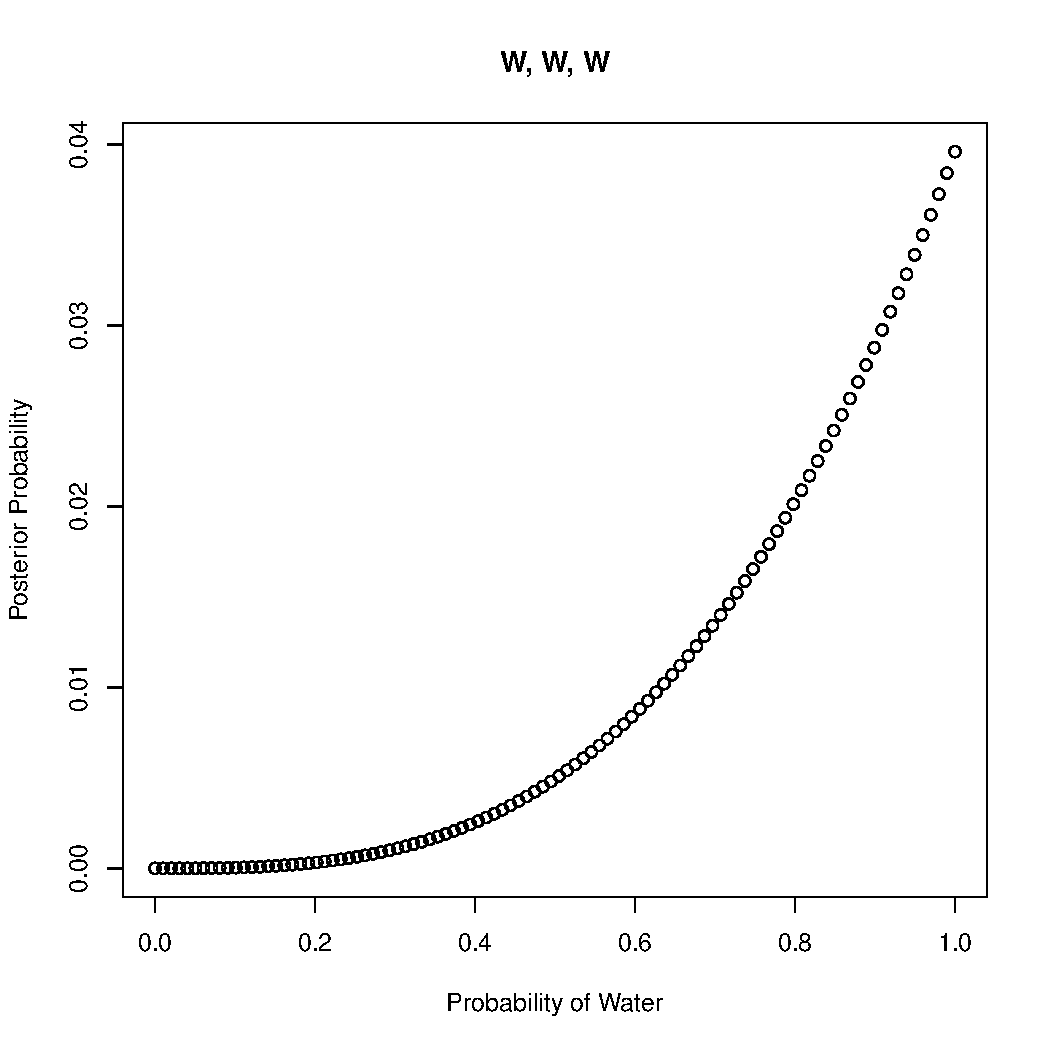
\includegraphics[width=\maxwidth]{figure/unnamed-chunk-2-1} 
\begin{kframe}\begin{alltt}
\hlcom{#W, W, W, L}

\hlstd{likelihood} \hlkwb{<-} \hlkwd{dbinom}\hlstd{(}\hlnum{3}\hlstd{,} \hlkwc{size} \hlstd{=} \hlnum{4}\hlstd{,} \hlkwc{prob} \hlstd{= p_grid)}

\hlstd{unstd.posterior} \hlkwb{<-} \hlstd{likelihood} \hlopt{*} \hlstd{prior}

\hlstd{posterior} \hlkwb{<-} \hlstd{unstd.posterior}\hlopt{/}\hlkwd{sum}\hlstd{(unstd.posterior)}

\hlkwd{plot}\hlstd{(p_grid, posterior,} \hlkwc{type} \hlstd{=} \hlstr{"b"}\hlstd{,} \hlkwc{xlab} \hlstd{=} \hlstr{"Probability of Water"}\hlstd{,}
     \hlkwc{ylab} \hlstd{=} \hlstr{"Posterior Probability"}\hlstd{,} \hlkwc{main} \hlstd{=} \hlstr{"W, W, W, L"}\hlstd{)}
\end{alltt}
\end{kframe}
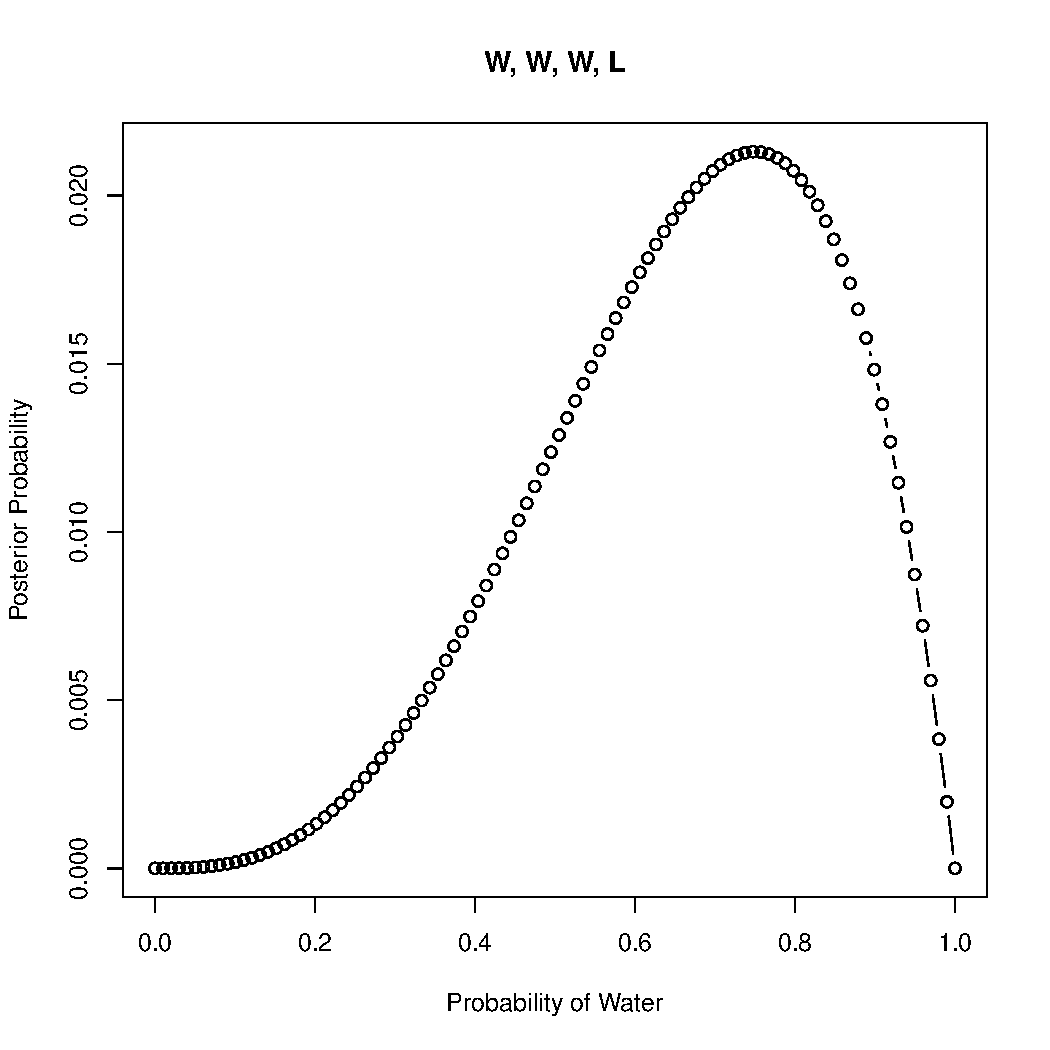
\includegraphics[width=\maxwidth]{figure/unnamed-chunk-2-2} 
\begin{kframe}\begin{alltt}
\hlcom{#L, W, W, L, W, W, W}

\hlstd{likelihood} \hlkwb{<-} \hlkwd{dbinom}\hlstd{(}\hlnum{5}\hlstd{,} \hlkwc{size} \hlstd{=} \hlnum{7}\hlstd{,} \hlkwc{prob} \hlstd{= p_grid)}

\hlstd{unstd.posterior} \hlkwb{<-} \hlstd{likelihood} \hlopt{*} \hlstd{prior}

\hlstd{posterior} \hlkwb{<-} \hlstd{unstd.posterior}\hlopt{/}\hlkwd{sum}\hlstd{(unstd.posterior)}

\hlkwd{plot}\hlstd{(p_grid, posterior,} \hlkwc{type} \hlstd{=} \hlstr{"b"}\hlstd{,} \hlkwc{xlab} \hlstd{=} \hlstr{"Probability of Water"}\hlstd{,}
     \hlkwc{ylab} \hlstd{=} \hlstr{"Posterior Probability"}\hlstd{,} \hlkwc{main} \hlstd{=} \hlstr{"L, W, W, L, W, W, W"}\hlstd{)}
\end{alltt}
\end{kframe}
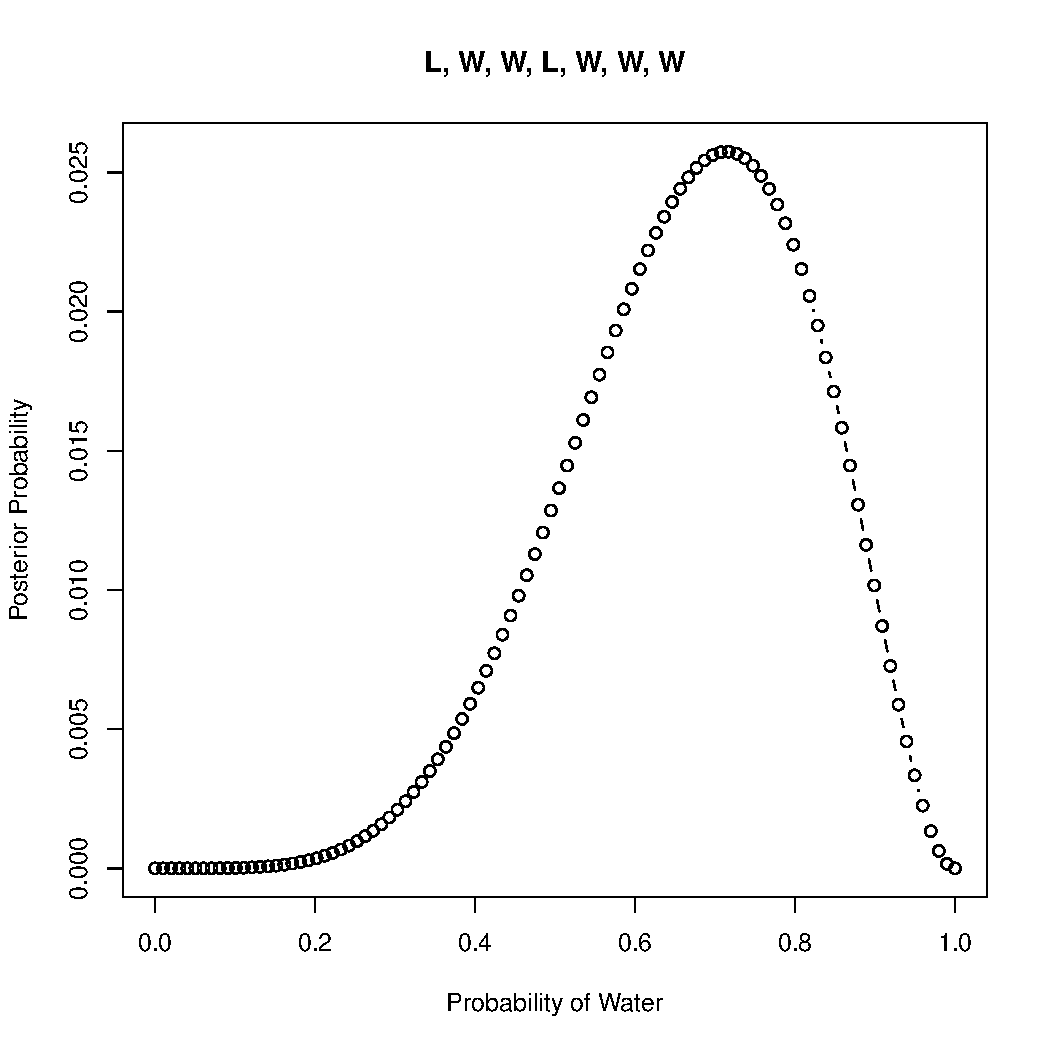
\includegraphics[width=\maxwidth]{figure/unnamed-chunk-2-3} 

\end{knitrout}

\begin{problem}{2M2}
\text{}\\
Now assume a prior for \textit{p} that is equal to zero when \textit{p} < 0.5 and is a positive constant when \textit{p} $\geq$ 0.5. Again compute and plot the grid approximate posterior distribution for each of the sets of observations in the problem just above.
\end{problem}

\begin{knitrout}
\definecolor{shadecolor}{rgb}{0.969, 0.969, 0.969}\color{fgcolor}\begin{kframe}
\begin{alltt}
\hlcom{#Grid of probability values}
\hlstd{p_grid} \hlkwb{<-} \hlkwd{seq}\hlstd{(}\hlkwc{from} \hlstd{=} \hlnum{0}\hlstd{,} \hlkwc{to} \hlstd{=} \hlnum{1}\hlstd{,} \hlkwc{length.out} \hlstd{=} \hlnum{100}\hlstd{)}

\hlcom{#P_grid values below 0.5 receive a 0 prior, }
\hlcom{#any p_grid value 0.5 or above is assigned a prior of 1}
\hlstd{prior} \hlkwb{<-} \hlkwd{ifelse}\hlstd{(p_grid} \hlopt{<} \hlnum{0.5}\hlstd{,} \hlnum{0}\hlstd{,} \hlnum{1}\hlstd{)}

\hlcom{#W, W, W}

\hlstd{likelihood} \hlkwb{<-} \hlkwd{dbinom}\hlstd{(}\hlnum{3}\hlstd{,} \hlkwc{size} \hlstd{=} \hlnum{3}\hlstd{,} \hlkwc{prob} \hlstd{= p_grid)}

\hlstd{unstd.posterior} \hlkwb{<-} \hlstd{likelihood} \hlopt{*} \hlstd{prior}

\hlstd{posterior} \hlkwb{<-} \hlstd{unstd.posterior}\hlopt{/}\hlkwd{sum}\hlstd{(unstd.posterior)}

\hlkwd{plot}\hlstd{(p_grid, posterior,} \hlkwc{type} \hlstd{=} \hlstr{"b"}\hlstd{,} \hlkwc{xlab} \hlstd{=} \hlstr{"Probability of Water"}\hlstd{,}
     \hlkwc{ylab} \hlstd{=} \hlstr{"Posterior Probability"}\hlstd{,} \hlkwc{main} \hlstd{=} \hlstr{"W, W, W"}\hlstd{)}
\end{alltt}
\end{kframe}
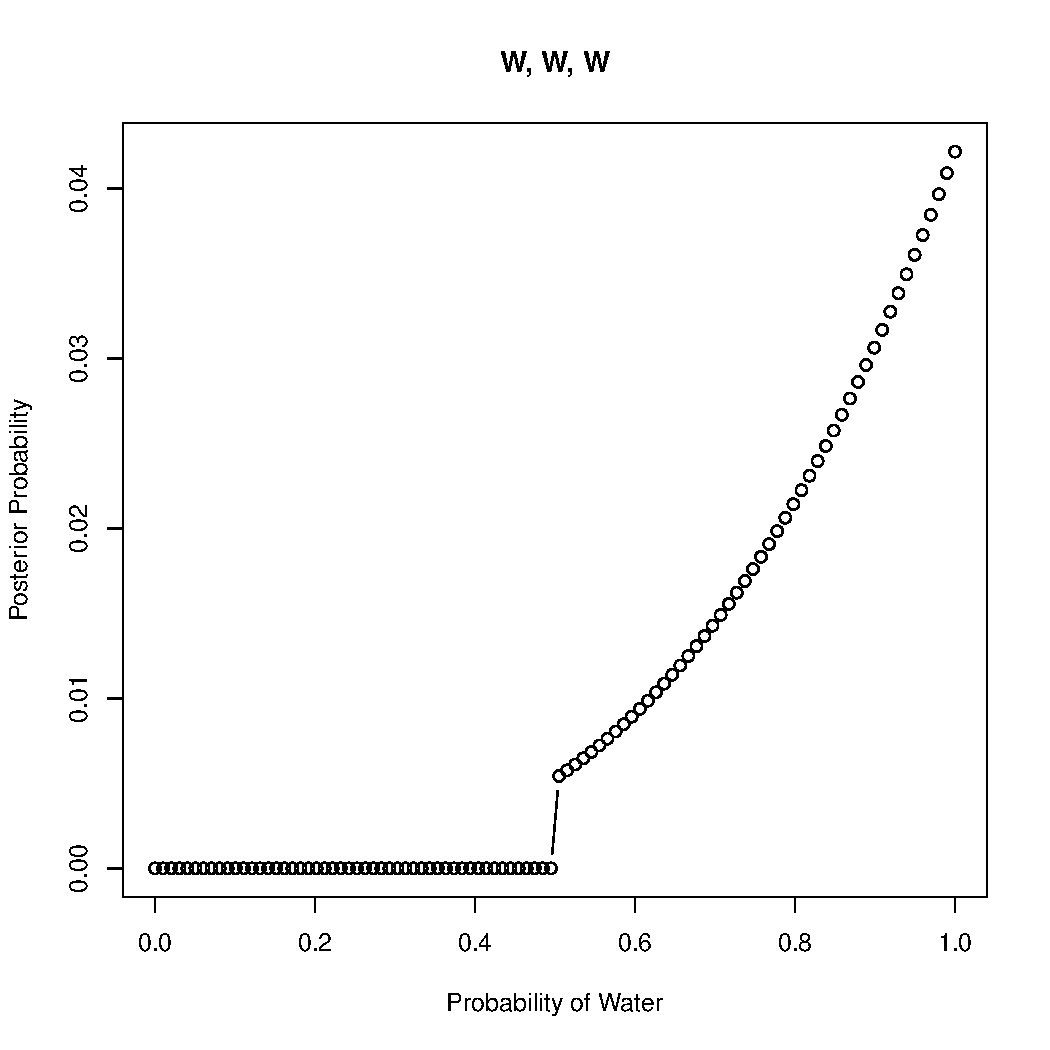
\includegraphics[width=\maxwidth]{figure/unnamed-chunk-3-1} 
\begin{kframe}\begin{alltt}
\hlcom{#W, W, W, L}

\hlstd{likelihood} \hlkwb{<-} \hlkwd{dbinom}\hlstd{(}\hlnum{3}\hlstd{,} \hlkwc{size} \hlstd{=} \hlnum{4}\hlstd{,} \hlkwc{prob} \hlstd{= p_grid)}

\hlstd{unstd.posterior} \hlkwb{<-} \hlstd{likelihood} \hlopt{*} \hlstd{prior}

\hlstd{posterior} \hlkwb{<-} \hlstd{unstd.posterior}\hlopt{/}\hlkwd{sum}\hlstd{(unstd.posterior)}

\hlkwd{plot}\hlstd{(p_grid, posterior,} \hlkwc{type} \hlstd{=} \hlstr{"b"}\hlstd{,} \hlkwc{xlab} \hlstd{=} \hlstr{"Probability of Water"}\hlstd{,}
     \hlkwc{ylab} \hlstd{=} \hlstr{"Posterior Probability"}\hlstd{,} \hlkwc{main} \hlstd{=} \hlstr{"W, W, W, L"}\hlstd{)}
\end{alltt}
\end{kframe}
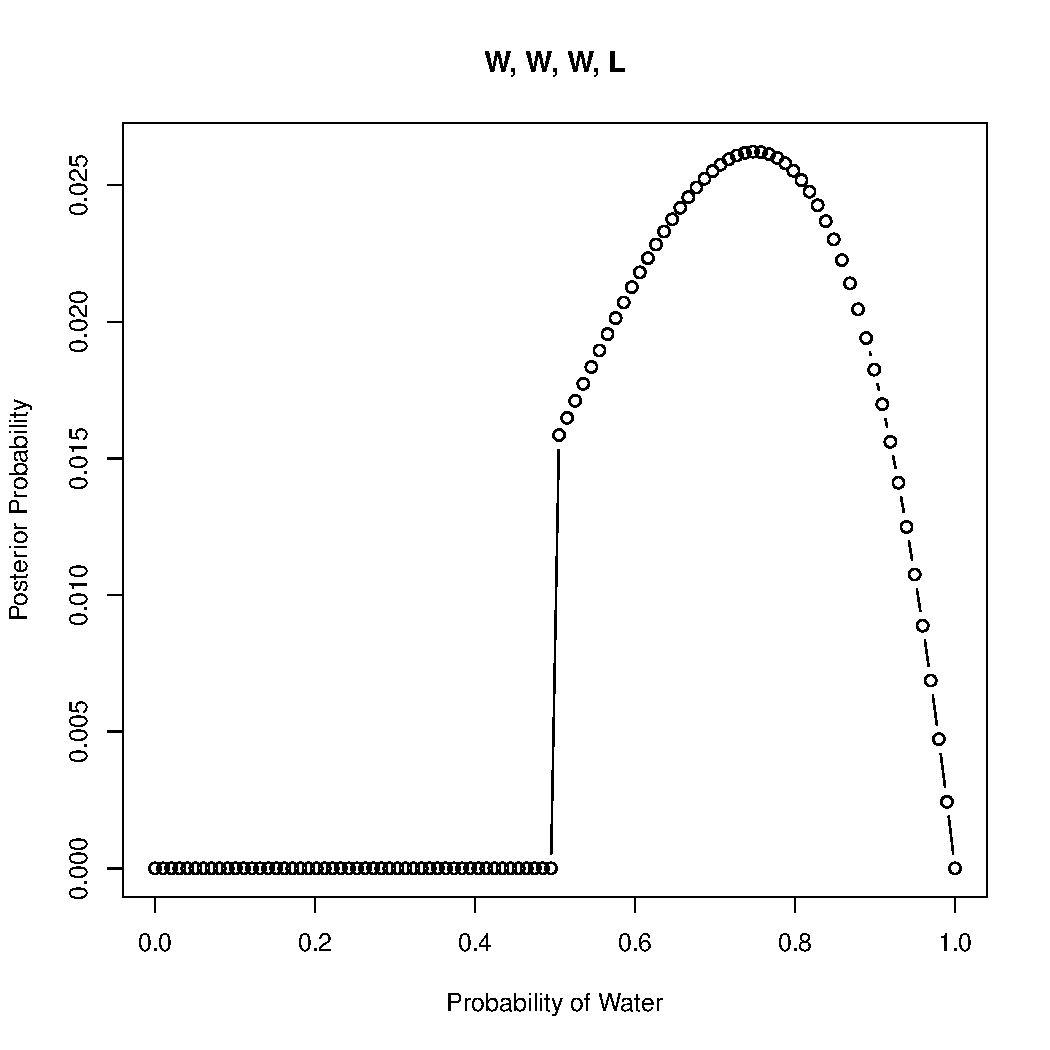
\includegraphics[width=\maxwidth]{figure/unnamed-chunk-3-2} 
\begin{kframe}\begin{alltt}
\hlcom{#L, W, W, L, W, W, W}

\hlstd{likelihood} \hlkwb{<-} \hlkwd{dbinom}\hlstd{(}\hlnum{5}\hlstd{,} \hlkwc{size} \hlstd{=} \hlnum{7}\hlstd{,} \hlkwc{prob} \hlstd{= p_grid)}

\hlstd{unstd.posterior} \hlkwb{<-} \hlstd{likelihood} \hlopt{*} \hlstd{prior}

\hlstd{posterior} \hlkwb{<-} \hlstd{unstd.posterior}\hlopt{/}\hlkwd{sum}\hlstd{(unstd.posterior)}

\hlkwd{plot}\hlstd{(p_grid, posterior,} \hlkwc{type} \hlstd{=} \hlstr{"b"}\hlstd{,} \hlkwc{xlab} \hlstd{=} \hlstr{"Probability of Water"}\hlstd{,}
     \hlkwc{ylab} \hlstd{=} \hlstr{"Posterior Probability"}\hlstd{,} \hlkwc{main} \hlstd{=} \hlstr{"L, W, W, L, W, W, W"}\hlstd{)}
\end{alltt}
\end{kframe}
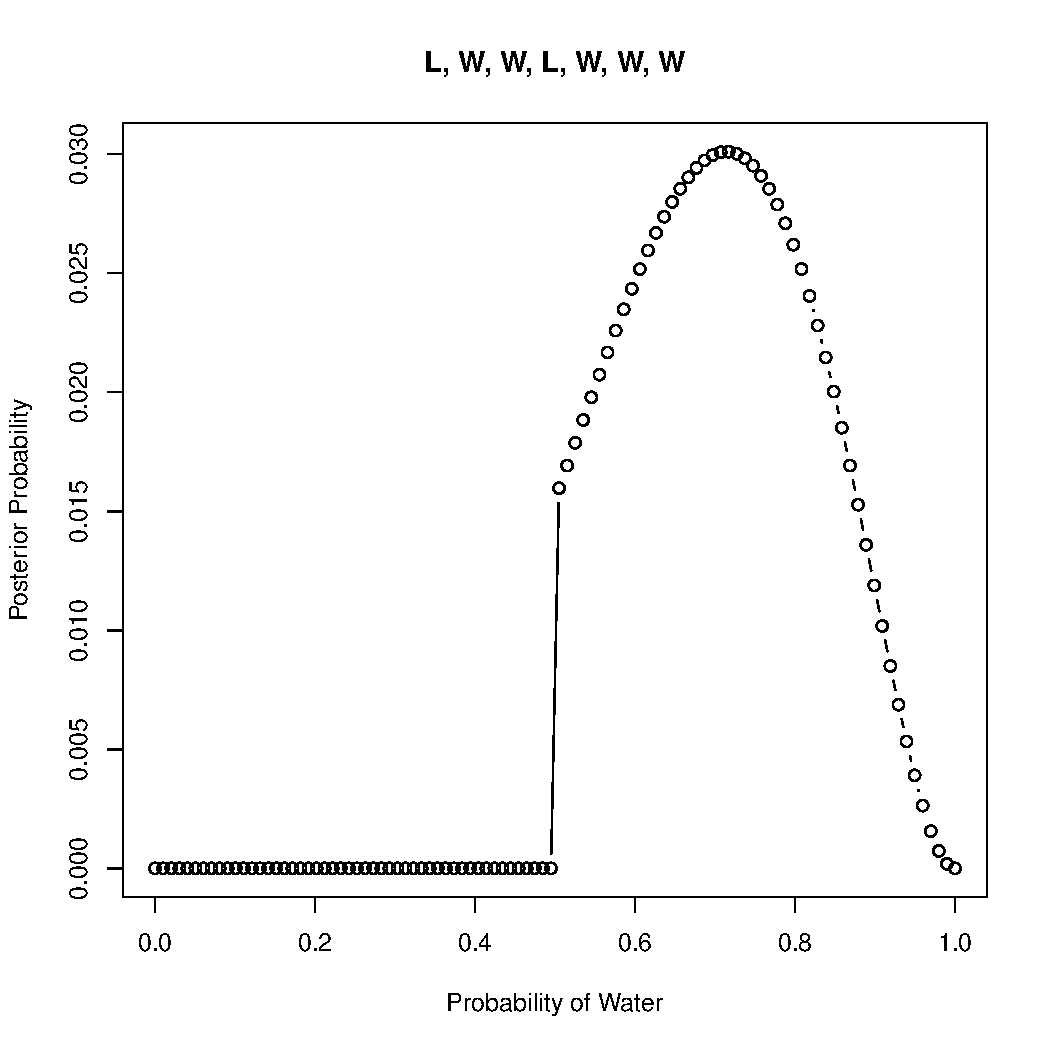
\includegraphics[width=\maxwidth]{figure/unnamed-chunk-3-3} 

\end{knitrout}

\begin{problem}{2M3}
\text{}\\
Suppose there are two globes, one for Earth and one for Mars. The Earth globe is 70\% covered in water. The Mars globe is 100\% land. Further, suppose that one of these globes - you don't know which - was tossed in the air and produced a "land" observation. Assume that each globe was equally likely to be tossed. Show that the posterior probability that the globe was the Earth, conditional on seeing "land" (Pr(Earth$\vert$land)), is 0.23.
\end{problem}

Pr(Earth$\vert$land) = $\textfrac{Pr(land$\vert$Earth)*Pr(Earth)}{Pr(land)}$ = $\textfrac{0.3*0.5}{0.3*0.5+1.0*0.5}$ $\approx$ 0.23

\begin{problem}{2M4}
\text{}\\
Suppose you have a deck with only three cards. Each card has two sides, and each side is either black or white. One card has two black sides. The second card has one black and one white side. The third card has two white sides. Now suppose all three cards are placed in a bag and shuffled. Someone reaches into the bag and pulls out a card and placed it flat on a table. A black side is shown facing up, but you don't know the color of the side facing down. Show that the probability that the other side is also black is 2/3. Use the counting method (Section 2 of the chapter) to approach the problem. This means counting up the ways that each card could produce the observed data (a black side facing up on the table).
\end{problem}

Scenarios:
\begin{enumerate}
  \item Up: Card 1, Side 1 (Black), Down: Card 1, Side 2 (Black)
  \item Up: Card 1, Side 2 (Black), Down: Card 1, Side 1 (Black)
  \item Up: Card 2, Side 1 (Black), Down: Card 2, Side 2 (White)
  \item Up: Card 2, Side 2 (White), Down: Card 2, Side 1 (Black)
  \item Up: Card 3, Side 1 (White), Down: Card 3, Side 2 (White)
  \item Up: Card 3, Side 2 (White), Down: Card 3, Side 1 (White)
\end{enumerate}

There are 3 possible scenarios where the side facing up is black (Scenarios 1, 2, \& 3). In two of these three scenarios, the other side of the card is also black. Thus, the probability that the other side is also black is 2/3.

\begin{problem}{2M5}
\text{}\\
Now suppose there are four cards: B/B, B/W, W/W, and another B/B. Again suppose a card is drawn from the bag and a black side appears face up. Again calculate the probability that the other side is black.
\end{problem}

Scenarios:
\begin{enumerate}
  \item Up: Card 1, Side 1 (Black), Down: Card 1, Side 2 (Black)
  \item Up: Card 1, Side 2 (Black), Down: Card 1, Side 1 (Black)
  \item Up: Card 2, Side 1 (Black), Down: Card 2, Side 2 (White)
  \item Up: Card 2, Side 2 (White), Down: Card 2, Side 1 (Black)
  \item Up: Card 3, Side 1 (White), Down: Card 3, Side 2 (White)
  \item Up: Card 3, Side 2 (White), Down: Card 3, Side 1 (White)
  \item Up: Card 4, Side 1 (Black), Down: Card 4, Side 2 (Black)
  \item Up: Card 4, Side 2 (Black), Down: Card 4, Side 1 (Black)
\end{enumerate}

There are 5 possible scenarios where the side facing up is black (Scenarios 1, 2, 3, 7, \& 8). In four of these five scenarios, the other side of the card is also black. Thus, the probability that the other side is also black is 4/5.

\begin{problem}{2M6}
\text{}\\
Imagine that black ink is heavy, and so cards with black sides are heavier than cards with white sides. As a result, it's less likely that a card with black sides is pulled from the bag. So again assume there are three cards: B/B, B/W, and W/W. After experimenting a number of times, you conlude that for every way to pull the B/B card from the bag, there are 2 ways to pull the B/W card and 3 ways to pull the W/W card. Again suppose that a card is pulled and a black side appears face up. Show that the probability the other side is black is now 0.5. Use the counting method, as before.
\end{problem}

Card 1 has 2 ways to produce the data, while Card 2 has 1 way (as shown in the scenarios in the previous questions). Adding in the multipliers, we now have Card 1 with 2*1 = 2 ways to produce the data and Card 2 with 1*2 = 2 ways to produce the data. Since the other side of Card 1 is always black and the other side of Card 2 is white if the black side is up, we have: \\

$\textfrac{2*1+0*2}{2*1+1*2}$ = $\textfrac{2}{4}$ = $\textfrac{1}{2}$

\begin{problem}{2M7}
\text{}\\
Assume again the original card problem, with a single card showing a black side face up. Before looking at the other side, we draw another card from the bag and lay it face up on the table. The face that is shown on the new card is white. Show that the probability that the first card, the one showing a black side, has black on its other side is now 0.75. Use the counting method, if you can. Hint: Treat this like the sequence of globe tosses, counting all the ways to see each observation, for each possible first card.
\end{problem}

Scenarios:
\begin{enumerate}
  \item Scenario 1
  \begin{itemize}
    \item Up: Card 1, Side 1 (Black), Down: Card 1, Side 2 (Black)
    \item Up: Card 2, Side 2 (White), Down: Card 2, Side 1 (Black)
  \end{itemize}
  \item Scenario 2
  \begin{itemize}
    \item Up: Card 1, Side 1 (Black), Down: Card 1, Side 2 (Black)
    \item Up: Card 3, Side 1 (White), Down: Card 3, Side 2 (White)
  \end{itemize}
  \item Scenario 3
  \begin{itemize}
    \item Up: Card 1, Side 1 (Black), Down: Card 1, Side 2 (Black)
    \item Up: Card 3, Side 2 (White), Down: Card 3, Side 1 (White)
  \end{itemize}
  \item Scenario 4
  \begin{itemize}
    \item Up: Card 1, Side 2 (Black), Down: Card 1, Side 1 (Black)
    \item Up: Card 2, Side 2 (White), Down: Card 2, Side 1 (Black)
  \end{itemize}
  \item Scenario 5
  \begin{itemize}
    \item Up: Card 1, Side 2 (Black), Down: Card 1, Side 1 (Black)
    \item Up: Card 3, Side 1 (White), Down: Card 3, Side 2 (White)
  \end{itemize}
  \item Scenario 6
  \begin{itemize}
    \item Up: Card 1, Side 2 (Black), Down: Card 1, Side 1 (Black)
    \item Up: Card 3, Side 2 (White), Down: Card 3, Side 1 (White)
  \end{itemize}
  \item Scenario 7
  \begin{itemize}
    \item Up: Card 2, Side 1 (Black), Down: Card 2, Side 2 (White)
    \item Up: Card 3, Side 1 (White), Down: Card 3, Side 2 (White)
  \end{itemize}
  \item Scenario 8
  \begin{itemize}
    \item Up: Card 2, Side 1 (Black), Down: Card 2, Side 2 (White)
    \item Up: Card 3, Side 2 (White), Down: Card 3, Side 1 (White)
  \end{itemize}
\end{enumerate}

As can be seen, there are 8 separate scenarios where the first card shows a black side and the second card shows a white side. In 6 out of 8 scenarios, the other side of the first card is also black. Thus, the probability that the other side of the first card is also black when the first card is showing black and the second card is showing white is: $\textfrac{6}{8}$ = 0.75.

\begin{problem}{2H1}
\text{}\\
Suppose there are two species of panda bear. Both are equally common in the wild and live in the same places. They look exactly alike and eat the same food, and there is yet no genetic assay capable of telling them apart. They differ however in their family sizes. Species A gives birth to twins 10\% of the time. otherwise birthing a single infant. Species B births twins 20\% of the time, otherwise birthing singleton infants. Assume these numbers are known with certainty, from many years of field research.

Now suppose you are managing a captive panda breeding program. You have a new female panda of unkown species, and she has just given birth to twins. What is the probability that her next birth will also be twins?
\end{problem}

\begin{knitrout}
\definecolor{shadecolor}{rgb}{0.969, 0.969, 0.969}\color{fgcolor}\begin{kframe}
\begin{alltt}
\hlstd{p_A} \hlkwb{=} \hlnum{1}\hlopt{/}\hlnum{2} \hlcom{# prior probability of species A}
\hlstd{p_B} \hlkwb{=} \hlnum{1}\hlopt{/}\hlnum{2} \hlcom{# prior probability of species B}

\hlstd{p_twins_A} \hlkwb{=} \hlnum{0.1} \hlcom{# P(Twins|Species = A)}
\hlstd{p_twins_B} \hlkwb{=} \hlnum{0.2} \hlcom{# P(Twins|Species = B)}

\hlcom{# Given first birth are twins, what is the probability that}
\hlcom{# second birth are also twins}


\hlcom{# Given a species, births should be independent. }
\hlcom{# But, because we are unsure about the species, we need to }
\hlcom{# average out the species to estimate the probability of}
\hlcom{# next birth being twins, given that the first birth }
\hlcom{# were twins.}

\hlcom{# In other words,if I knew the species, knowing that the current }
\hlcom{# birth resulted in twins, would not change my expectation about }
\hlcom{# twins for the following birth.}

\hlcom{# Thus, in principle:}
\hlcom{# P(twins) = P(twins|Species = A)P(A) + P(twins|Species = B)P(B)}

\hlcom{# However, knowing about a single twin birth, does change }
\hlcom{# the relative plausibilities of the two species. So, P(A) and}
\hlcom{# P(B), are actually P(A|twins) and P(B|twins).}

\hlcom{# Thus, we are actually looking for:}
\hlcom{# P(twins) = P(twins|A)*P(A|twins) + P(twins|B)*P(B|twins)}

\hlcom{# P(A|twins) = P(twins|A)P(A)/P(twins)}
\hlcom{# P(B|twins) = P(twins|B)P(B)/P(twins)}
\hlcom{# P(twins) = P(twins|A)P(A) + P(twins|B)P(B)}
\hlstd{p_twins_unadjusted} \hlkwb{=} \hlnum{0.1} \hlopt{*} \hlnum{0.5} \hlopt{+} \hlnum{0.2} \hlopt{*} \hlnum{0.5}

\hlstd{p_A_twins} \hlkwb{=} \hlstd{(}\hlnum{0.1} \hlopt{*} \hlnum{0.5}\hlstd{)}\hlopt{/}\hlstd{p_twins_unadjusted}
\hlstd{p_B_twins} \hlkwb{=} \hlstd{(}\hlnum{0.2} \hlopt{*} \hlnum{0.5}\hlstd{)}\hlopt{/}\hlstd{p_twins_unadjusted}

\hlstd{p_twins_adjusted} \hlkwb{=} \hlnum{0.1} \hlopt{*} \hlstd{p_A_twins} \hlopt{+} \hlnum{0.2} \hlopt{*} \hlstd{p_B_twins}
\hlkwd{print}\hlstd{(p_twins_adjusted)}
\end{alltt}
\begin{verbatim}
## [1] 0.1666667
\end{verbatim}
\end{kframe}
\end{knitrout}

Thus, Pr(twins) $\approx$ 0.167.

\begin{problem}{2H2}
\text{}\\
Recall all the facts from the problem above. Now compute the probability that the panda we have is from species A, assuming we have obeserved only the first birth and that it is twins.
\end{problem}

\begin{knitrout}
\definecolor{shadecolor}{rgb}{0.969, 0.969, 0.969}\color{fgcolor}\begin{kframe}
\begin{alltt}
\hlcom{# P(A|twins) = P(twins|A)P(A)/P(twins)}

\hlstd{p_twins} \hlkwb{=} \hlnum{0.1} \hlopt{*} \hlnum{0.5} \hlopt{+} \hlnum{0.2} \hlopt{*} \hlnum{0.5}

\hlstd{p_A_twins} \hlkwb{=} \hlstd{(}\hlnum{0.1} \hlopt{*} \hlnum{0.5}\hlstd{)}\hlopt{/}\hlstd{p_twins}

\hlkwd{print}\hlstd{(p_A_twins)}
\end{alltt}
\begin{verbatim}
## [1] 0.3333333
\end{verbatim}
\end{kframe}
\end{knitrout}

Thus, Pr(A$\vert$twins) $\approx$ 0.33.

\begin{problem}{2H3}
\text{}\\
Continuing on from the previous problem, suppose the same panda mother has a second birth and that it is not twins, but a singleton infant. Compute the posterior probability that this panda is species A.
\end{problem}

\begin{knitrout}
\definecolor{shadecolor}{rgb}{0.969, 0.969, 0.969}\color{fgcolor}\begin{kframe}
\begin{alltt}
\hlcom{# First birth = Twins}
\hlcom{# Second birth = Singleton}
\hlcom{# P(Species = A| Twins, Singleton)?}

\hlcom{# P(Species = A | Twins, Singleton) = P(Twins | Species = A) *}
\hlcom{#                                   P(Singleton | Species = A) *}
\hlcom{#                                      P(A) /}
\hlcom{#                                         P(Twins,Singleton)}
\hlcom{# P(Twins,Singleton) =  P(Twins | Species = A) *}
\hlcom{#                       P(Singleton | Species = A) *}
\hlcom{#                          P(A) +}
\hlcom{#                    P(Twins | Species = B) *}
\hlcom{#                       P(Singleton | Species = B) *}
\hlcom{#                          P(B)}

\hlstd{p_A_twins_singleton} \hlkwb{=} \hlstd{(} \hlnum{0.1} \hlopt{*} \hlnum{0.9} \hlopt{*} \hlnum{0.5}\hlstd{)} \hlopt{/}
                      \hlstd{((} \hlnum{0.1} \hlopt{*} \hlnum{0.9} \hlopt{*} \hlnum{0.5}\hlstd{)} \hlopt{+}
                            \hlstd{(} \hlnum{0.2} \hlopt{*} \hlnum{0.8} \hlopt{*} \hlnum{0.5} \hlstd{))}

\hlkwd{print}\hlstd{(p_A_twins_singleton)}
\end{alltt}
\begin{verbatim}
## [1] 0.36
\end{verbatim}
\end{kframe}
\end{knitrout}

Thus, Pr(A$\vert$twins, singleton) = 0.36.

\begin{problem}{2H4}
\text{}\\
A common boast of Bayesian statisticians is that Bayesian inference makes it easy to use all of the data, even if the data are of different types.
So suppose now that a veterinarian comes along who has a new genetic test that she claims can identify the species of our mother panda. But the test, like all tests, is imperfect. This is the information about the test:
\begin{itemize}
  \item The probability it correctly identifies a species A panda is 0.8.
  \item The probability it correctly identifies a species B panda is 0.65.
\end{itemize}
The vet administers the test to your panda and tells you that the test is positive for species A. First ignore your previous information from the births and compute the posterior probability that your panda is species A. Then redo your calculation, now using the birth data as well.
\end{problem}

\begin{knitrout}
\definecolor{shadecolor}{rgb}{0.969, 0.969, 0.969}\color{fgcolor}\begin{kframe}
\begin{alltt}
\hlcom{# Probability of species A given a postive genetic test for A?}

\hlcom{# P(test = A | Species = A) = 0.80}
\hlcom{# P(test = B | Species = A) = 0.20}
\hlcom{# P(test = B | Species = B) = 0.65}
\hlcom{# P(test = A | Species = B) = 0.35}

\hlcom{# P(Species = A | Test = A) =}
\hlcom{#   P(Test = A | Species = A) * P(Species = A) / P(Test = A)}

\hlcom{#P(test = A) = }
\hlcom{#   P(test = A | Species = A) * P(Species = A) + }
\hlcom{#   P(test = A | Species = B) * P(Species = B)}

\hlstd{p_a_testA} \hlkwb{=} \hlnum{0.8} \hlopt{*} \hlnum{0.5} \hlopt{/} \hlstd{(}\hlnum{0.8}\hlopt{*}\hlnum{0.5}\hlopt{+}\hlnum{0.35}\hlopt{*}\hlnum{0.5}\hlstd{)}

\hlkwd{print}\hlstd{(p_a_testA)}
\end{alltt}
\begin{verbatim}
## [1] 0.6956522
\end{verbatim}
\end{kframe}
\end{knitrout}

Thus, Pr(A$\vert$Test = A) $\approx$ 0.696.

\begin{knitrout}
\definecolor{shadecolor}{rgb}{0.969, 0.969, 0.969}\color{fgcolor}\begin{kframe}
\begin{alltt}
\hlcom{# P(Species = A | test = A, twins, singleton)?}

\hlcom{# P(Species = A | test = A, twins, singleton) =}
\hlcom{#               P(test = A | Species = A) *}
\hlcom{#               P(twins | Species = A) *}
\hlcom{#               P(singleton | Species = A) *}
\hlcom{#               P(Species = A) \textbackslash{}}
\hlcom{#               P(test = A, twins, singleton)}

\hlcom{# P(test = A, twins, singleton) =}
\hlcom{#               P(test = A | Species = A) *}
\hlcom{#               P(twins | Species = A) *}
\hlcom{#               P(singleton | Species = A) *}
\hlcom{#               P(Species = A) +}
\hlcom{#               P(test = A | Species = B) *}
\hlcom{#               P(twins | Species = B) *}
\hlcom{#               P(singleton | Species = B) *}
\hlcom{#               P(Species = B)}

\hlcom{# The individual probabilities are only conditional on}
\hlcom{# species being equal to A because otherwise they are}
\hlcom{# independent. A test = A does not depend on births, and}
\hlcom{# births should be independent.}

\hlstd{p_testA_twins_singleton} \hlkwb{=} \hlnum{0.8} \hlopt{*} \hlnum{0.1} \hlopt{*} \hlnum{0.9} \hlopt{*} \hlnum{0.5} \hlopt{+}
                        \hlnum{0.35} \hlopt{*} \hlnum{0.2} \hlopt{*} \hlnum{0.8} \hlopt{*} \hlnum{0.5}

\hlstd{p_A_testA_twins_singleton} \hlkwb{=} \hlstd{(}\hlnum{0.8} \hlopt{*} \hlnum{0.1} \hlopt{*} \hlnum{0.9} \hlopt{*} \hlnum{0.5}\hlstd{)} \hlopt{/} \hlstd{p_testA_twins_singleton}

\hlkwd{print}\hlstd{(p_A_testA_twins_singleton)}
\end{alltt}
\begin{verbatim}
## [1] 0.5625
\end{verbatim}
\end{kframe}
\end{knitrout}

Thus, Pr(A$\vert$Test = A, twins, singleton) = 0.5625.

\end{document}
